% debut d'un fichier latex standard
\documentclass[a4paper,12pt,twoside]{article}

% pour l'inclusion de figures en eps,pdf,jpg
\usepackage{graphicx}
\usepackage{subcaption}
\usepackage{wrapfig}
\usepackage{siunitx} % pour utiliser les unités SI. Commande à utiliser: \SI{quantité}{unité}
% quelques symboles mathematiques en plus
\usepackage{amsmath}
% le tout en langue francaise
\usepackage[french]{babel}
% on peut ecrire directement les caracteres avec l'accent
% a utiliser sur Linux/Windows
\usepackage[utf8]{inputenc}
\usepackage[T1]{fontenc}
% a utiliser sur le Mac
%\usepackage[applemac]{inputenc}
% pour l'inclusion de links dans le document 
\usepackage[colorlinks,bookmarks=false,linkcolor=blue,urlcolor=blue]{hyperref}

\paperheight=297mm
\paperwidth=210mm

\setlength{\textheight}{235mm}
\setlength{\topmargin}{-1.2cm} % pour centrer la page verticalement
%\setlength{\footskip}{5mm}
\setlength{\textwidth}{15cm}
\setlength{\oddsidemargin}{0.56cm}
\setlength{\evensidemargin}{0.56cm}

\pagestyle{plain}

% quelques abreviations utiles
\def \be {\begin{equation}}
\def \ee {\end{equation}}
\def \dd  {{\rm d}}

\newcommand{\mail}[1]{{\href{mailto:#1}{#1}}}
\newcommand{\ftplink}[1]{{\href{ftp://#1}{#1}}}
%
% latex SqueletteRapport.tex      % compile la source LaTeX
% xdvi SqueletteRapport.dvi &     % visualise le resultat
% dvips -t a4 -o SqueletteRapport.ps SqueletteRapport % produit un PostScript
% ps2pdf SqueletteRapport.ps      % convertit en pdf

% pdflatex SqueletteRapport.pdf    % compile et produit un pdf

% ======= Le document commence ici ======

\begin{document}
% Le titre, l'auteur et la date
\title{De la Terre à la Lune\\{\small Physique Numérique I}\\{\small Rapport 1}}
\date{\today}
\author{Delphine Martres et Damien Korber\\{\small \mail{delphine.martres@epfl.ch} et \mail{damien.korber@epfl.ch}}}
\maketitle
\tableofcontents % Table des matieres

% Quelques options pour les espacements entre lignes, l'identation 
% des nouveaux paragraphes, et l'espacement entre paragraphes
\baselineskip=16pt
\parindent=15pt
\parskip=5pt



%%%% ON COMMENCE A ECRIRE D'ICI

\section{Introduction}
Le roman de Jules Vernes \textit{"De la Terre à la Lune"} décrit une méthode originale pour envoyer des projectiles jusqu'à la lune à l'aide d'un canon. Cette rapport se concentre donc sur une analyse de la situation, en négligeant tout aspects de rotations. Ainsi, le rapport se concentre donc sur une analyse unidimensionelle du problème.

\section{Modélisation}
Dans ce projet, nous avons modélisé une terre et une lune sur une droite. Le centre de la terre se situe à l'origine de cette droite. Depuis la surface de la terre, un projectile est envoyé à une certaine vitesse vers la lune. Nous considérerons le cas où l'atmosphère terrestre n'a aucune influence sur le projectile, et le cas où elle a une influence.

\section{Solutions analytiques}
Dans la question a), il nous est demandé d'établir une équation différentielle régissant notre problème. Après plusieurs étapes de calcul faiblement pertinentes pour ce rapport, nous sommes arrivés à l'équation suivante.

\begin{equation}
    \frac{d}{dt}
    \begin{pmatrix}
        z \\
        \dot{z}
    \end{pmatrix}
    =
    \begin{pmatrix}
    \dot{z} \\
    G\cdot\frac{m_L}{(z_L - z)^2} - G\cdot\frac{m_T}{z^2} + \frac{\rho_0}{m}\cdot e^{-\frac{z-z_0}{\lambda}}\cdot S\cdot C_x\cdot \frac{\dot{z}^2}{2}
    \end{pmatrix}
    \label{eq:sol}
\end{equation}

Cette solution nous permet donc de décrire la trajectoire du projectile, dans son periple entre la terre et la lune. Cette solution comprend l'attraction de la terre et de la lune sur l'objet. De plus, elle comprend une force de frottement visqueuse, qui ralenti le projectile lors de son passage dans l'atmosphère.\\
\newline
Dans la question b), il est demandé de trouver le point d'équilibre de l'objet, s'il était statique. Pour obtenir la solution, nous avons simplement égalisé les forces gravitationnelles appliquées sur le projectile, et isolé $z$. Avec les valeurs fournies par le professeur, nous sommes arrivés au résultat suivant.

\begin{equation}
    z_E = \SI{3.460d8}{\meter}
    \label{val:zE}
\end{equation}

Finalement, dans la question c), il nous est demandé de trouver, en négligeant l'atmosphère terrestre, la vitesse initiale qu'il faudrait pour que le projectile s'arrête sur le point d'équilibre. A VERIFIER. Pour obtenir ce résultat, nous avons utilisé la conservation de l'énergie mécanique. Nous avons donc considéré l'énergie mécanique du projectile lorsqu'il se trouve sur terre, et lorsqu'il atteint le point d'équilibre. Sur terre, juste après le décolage, l'énergie du projectile se découpe en trois parties: Les potentielles gravitationnelles de la terre et de la lune, et l'énergie cinétique du projectile. Au point d'équilibre, il ne reste plus que les potentielles gravitationnelles, car l'objet est à l'arrêt. Ainsi, en isolant la vitesse, en utilisant les données du rapport et la position $z_E$ trouvée précédemment, nous sommes arrivé à ce résultat.

\begin{equation}
    v_0 = \SI{1.107d4}{\meter\per\second}
    \label{val:v0}
\end{equation}


\section{Résultats des simulations et réponses aux questions}
La deuxième partie de ce rapport se concentre sur l'implémentation numérique de ce problème afin de répondre aux questions posées. À l'aide d'un schéma de Euler, nous avons résolu numériquement l'équation différentielle et simulé, avec plusieurs pas de temps, notre problème.

\subsection{Question A - Simulation sans atmosphère}
Dans un premier temps, le système est simulé sur une durée de 24 heures en négligeant les effets de l'atmosphère.

%\begin{wrapfigure}{R}{0.55\textwidth}
%	\vspace{-20pt}
%    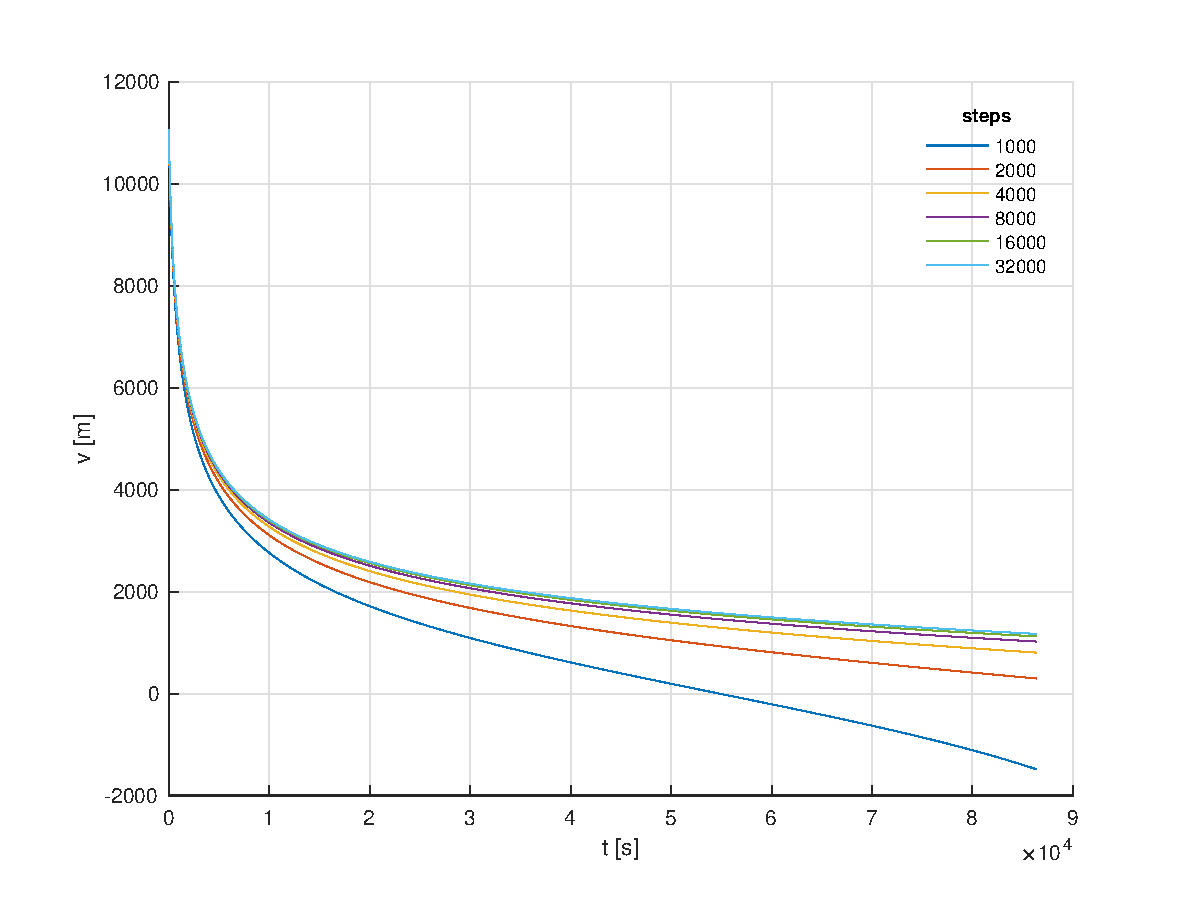
\includegraphics[width=0.53\textwidth]{graphs/vA.eps}
%    \vspace{-15pt}
%    \caption{Vitesse en fonction du temps}
%    \vspace{-10pt}
%    \label{fig:A-vt}
%\end{wrapfigure}

\begin{figure}[h]
	\centering
    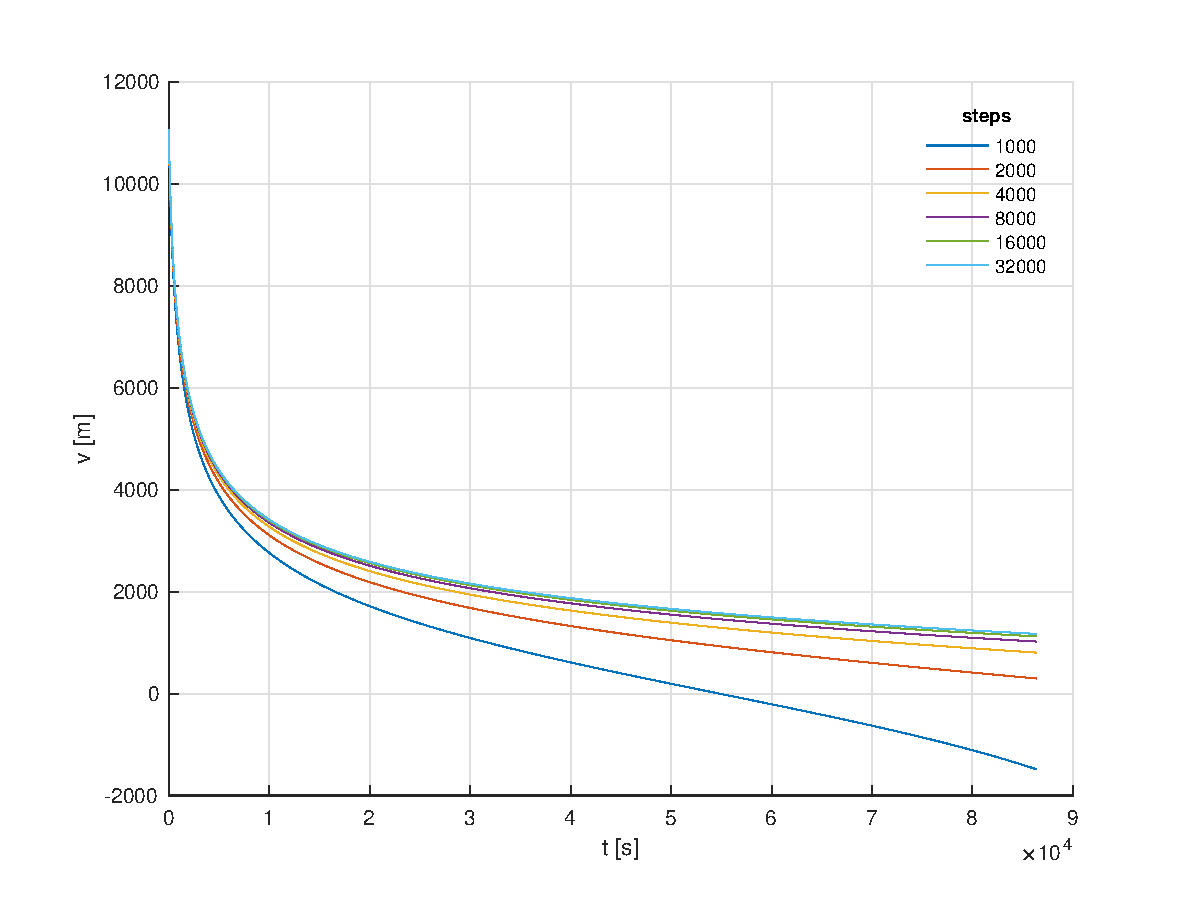
\includegraphics[width=0.53\textwidth]{graphs/vA.eps}
    \caption{Vitesse en fonction du temps}
    \label{fig:A-vt}
\end{figure}

On constate sur la figure \ref{fig:A-vt} que la vitesse diminue fortement au début de la simulation, en réponse à l'attraction terrestre, jusqu'à atteindre \SI{3500}{\meter\per\second} au bout de 3 heures, puis diminue beaucoup plus lentement après que le vaisseau se soit suffisamment éloigné de la Terre.\\

%\begin{wrapfigure}{L}{0.55\textwidth}
%	\vspace{-20pt}
%	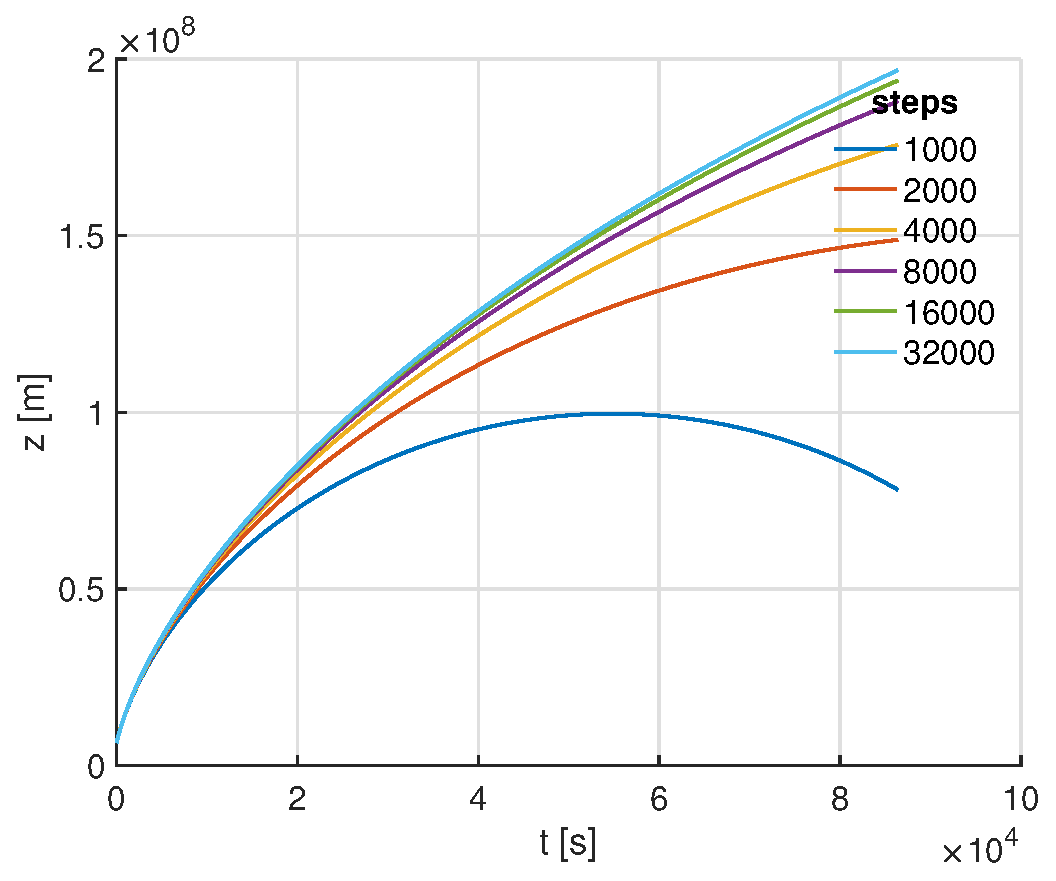
\includegraphics[width=0.53\textwidth]{graphs/zA.eps}
%	\vspace{-15pt}
%	\caption{Position en fonction du temps}
%	\vspace{-10pt}
%	\label{fig:A-zt}
%\end{wrapfigure}

\begin{figure}[h]
	\centering
	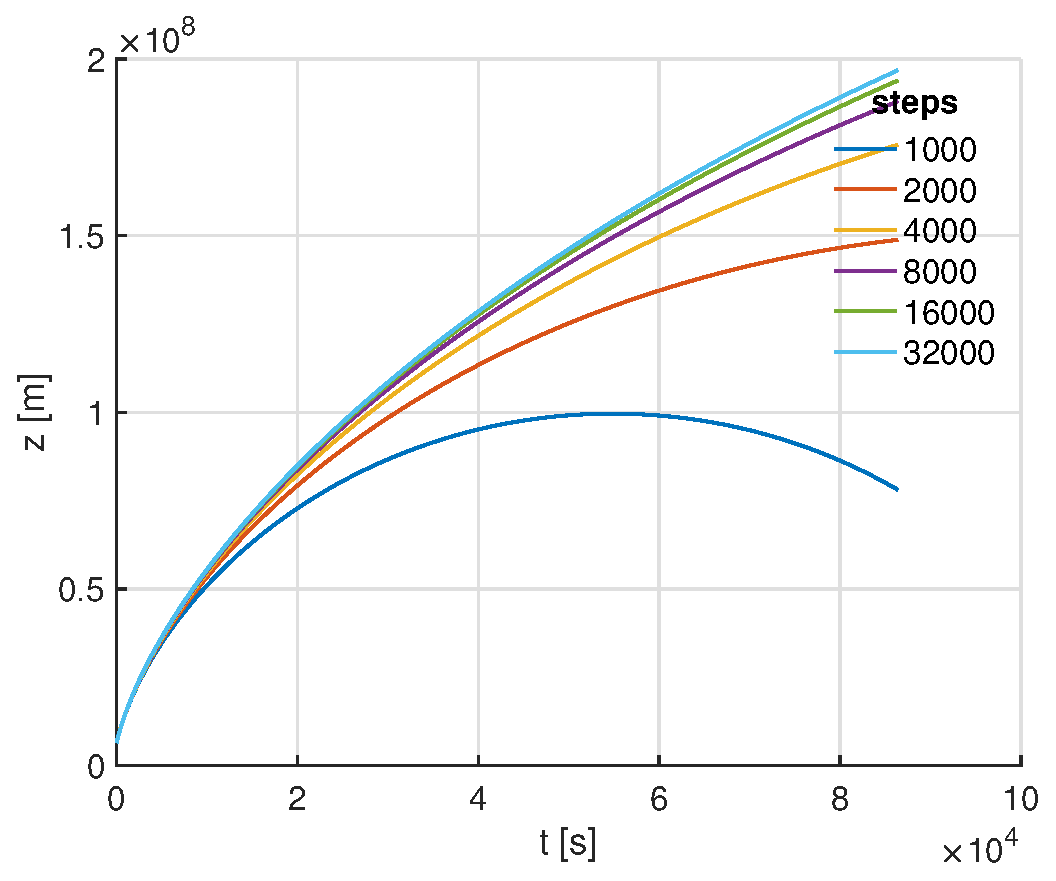
\includegraphics[width=0.53\textwidth]{graphs/zA.eps}
	\caption{Position en fonction du temps}
	\label{fig:A-zt}
\end{figure}

La figure \ref{fig:A-zt} montre que l'intégration par la méthode d'Euler est susceptible à de fortes imprécisions en-dessous d'un certain nombre de pas; en effet, dans la simulation avec nsteps=1000, la distance au point de départ diminue après 15 heures de vol, alors que cela n'est pas possible dans la réalité puisque l'accélération est toujours positive dans ce système.\\

\begin{figure}[h]
	\centering
	\begin{subfigure}[b]{0.45\textwidth}
		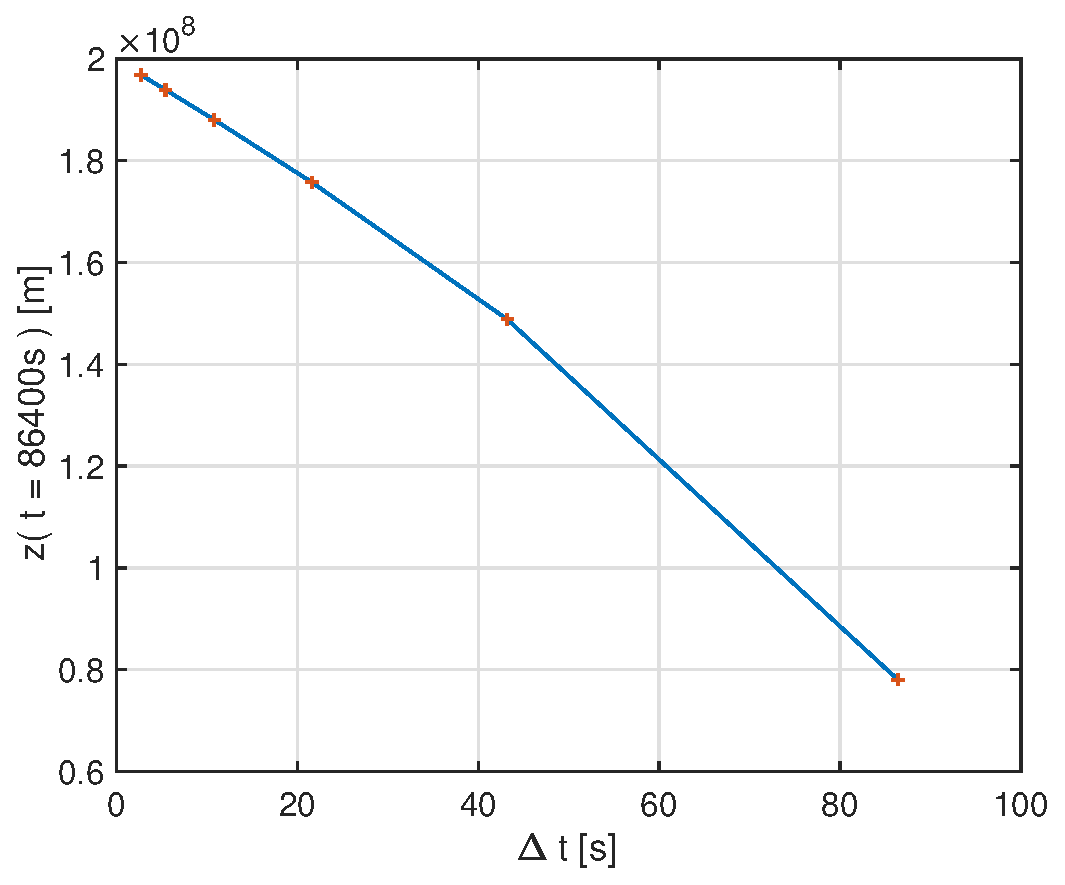
\includegraphics[width=\textwidth]{graphs/zConvA.eps}
		\caption{Graphique de convergence de la position}
		\label{fig:A-zConv}
	\end{subfigure}
	~
	\begin{subfigure}[b]{0.45\textwidth}
		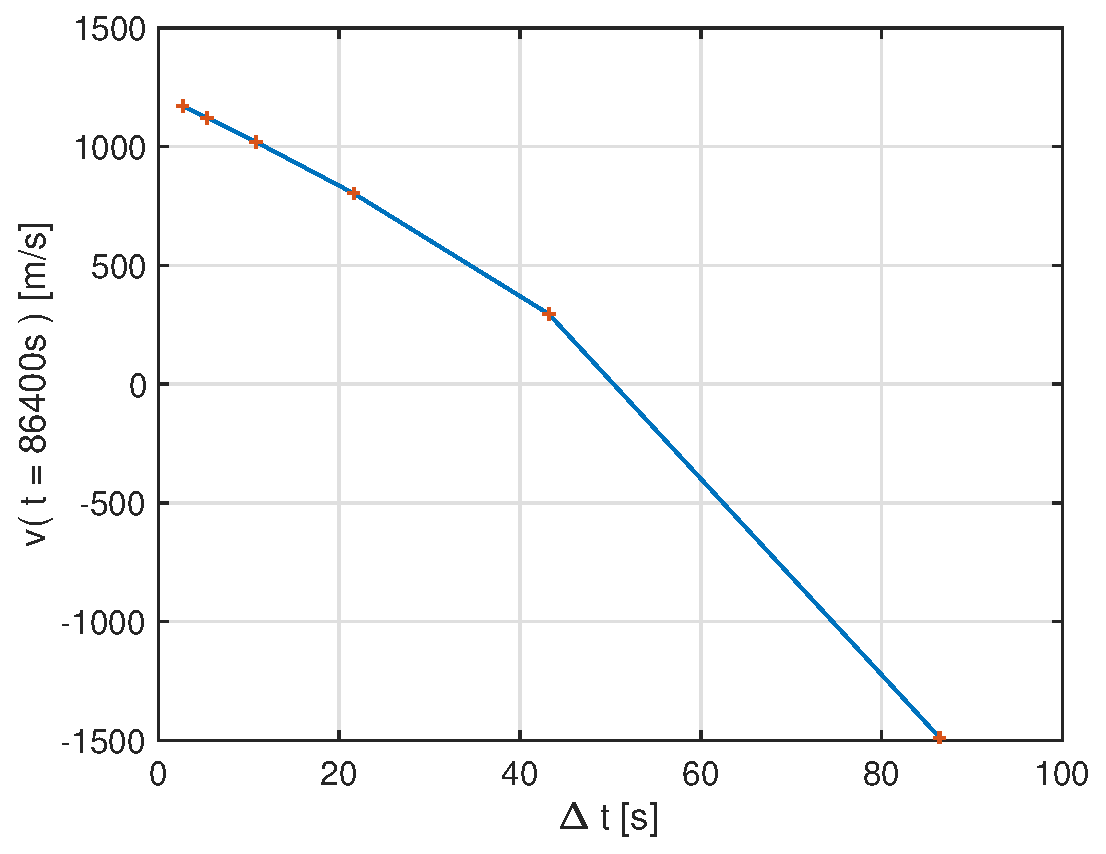
\includegraphics[width=\textwidth]{graphs/vConvA.eps}
		\caption{Graphique de convergence de la vitesse}
		\label{fig:A-vConv}
	\end{subfigure}
	\caption{Graphiques d'étude de convergence}
	\label{fig:A-conv}
\end{figure}

\subsection{Question B - Simulation avec atmosphère}
Dans cette deuxième question, nous nous intéressons à la traversée de l'atmosphère, avec différents pas-de-temps. Voici donc le résultat de ces simulations, durant les 10 premières secondes du décollage.\\

\begin{figure}[h]
	\centering
    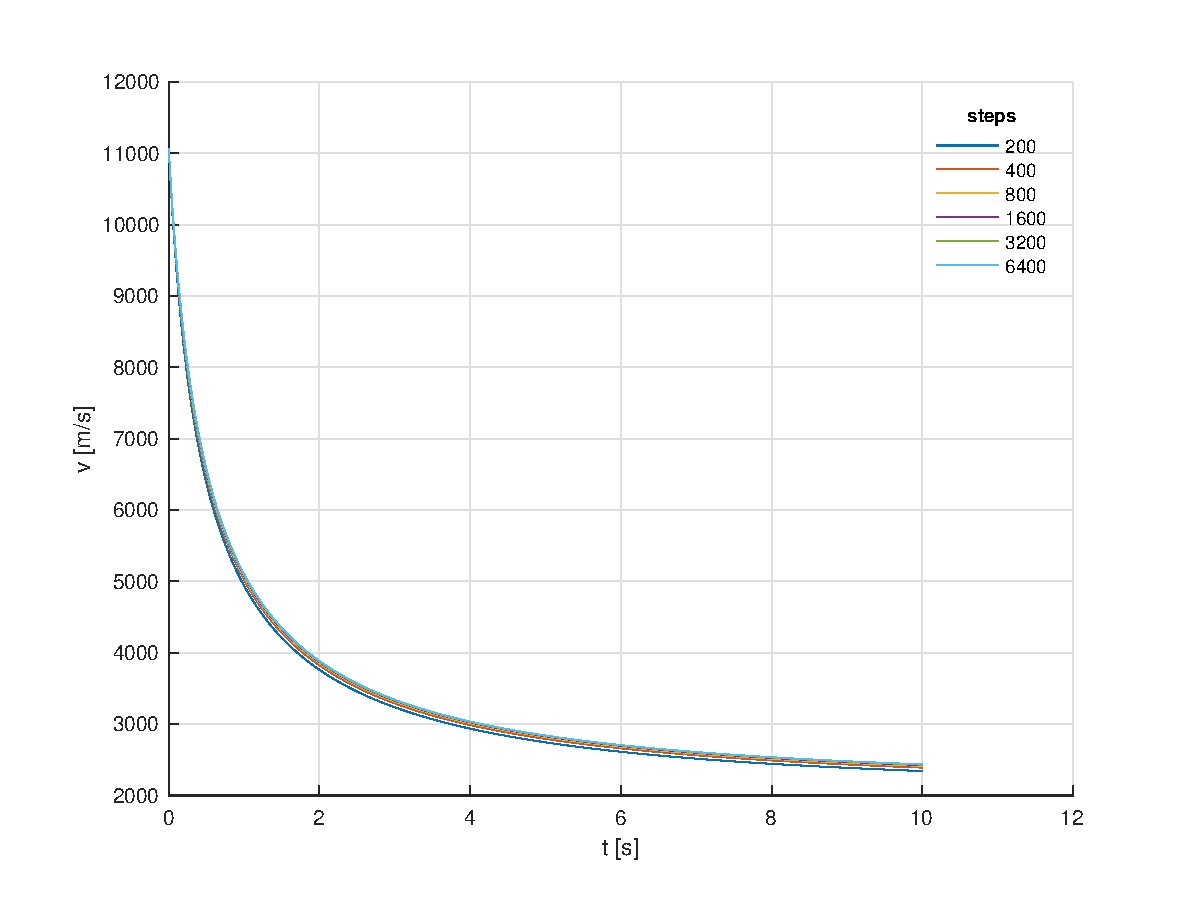
\includegraphics[width=0.53\textwidth]{graphs/vB.eps}
    \caption{Vitesse en fonction du temps}
    \label{fig:B-vt}
\end{figure}

La premier point intéressant est la vitesse du projectile. Le projectile est très fortement ralenti par l'atmosphère, et cela se ressent sur la figure \ref{fig:B-vt}. Dans toutes les simulations, la vitesse suit plus ou moins la même courbe. Au bout des 10 secondes de vol, le projectile a une vitesse d'environ \SI{2500}{\meter\per\second}. Cela s'explique par la vitesse au carrée de l'équation \ref{eq:sol}, dans le terme aérodynamique. En effet, la vitesse initiale $v0$ est tellement titanesque lors du décollage, et se ressent vraiment dans l'équation.\\

%\begin{wrapfigure}{L}{0.55\textwidth}
%	\vspace{-20pt}
%	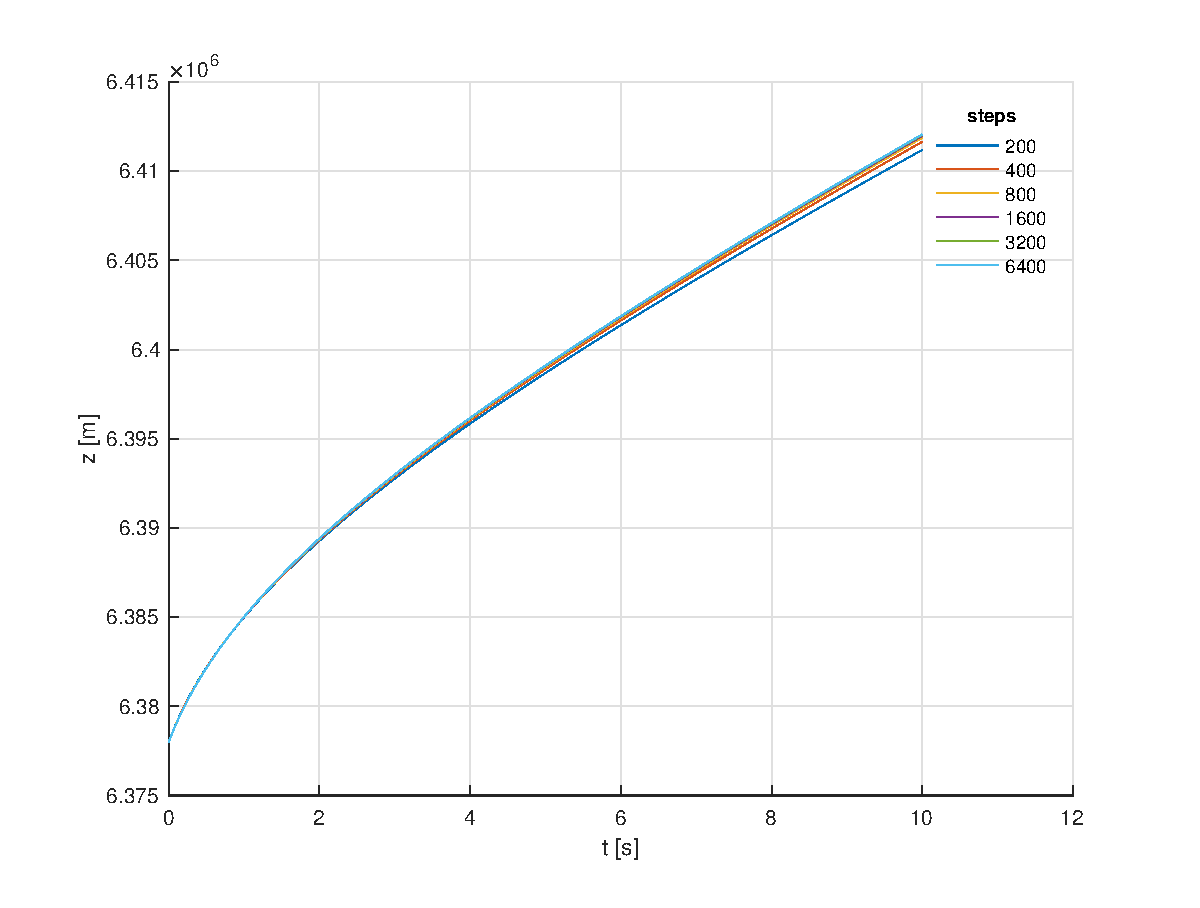
\includegraphics[width=0.53\textwidth]{graphs/zB.eps}
%	\vspace{-15pt}
%	\caption{Position en fonction du temps}
%	\vspace{-10pt}
%	\label{fig:B-zt}
%\end{wrapfigure}

\begin{figure}[h]
	\centering
	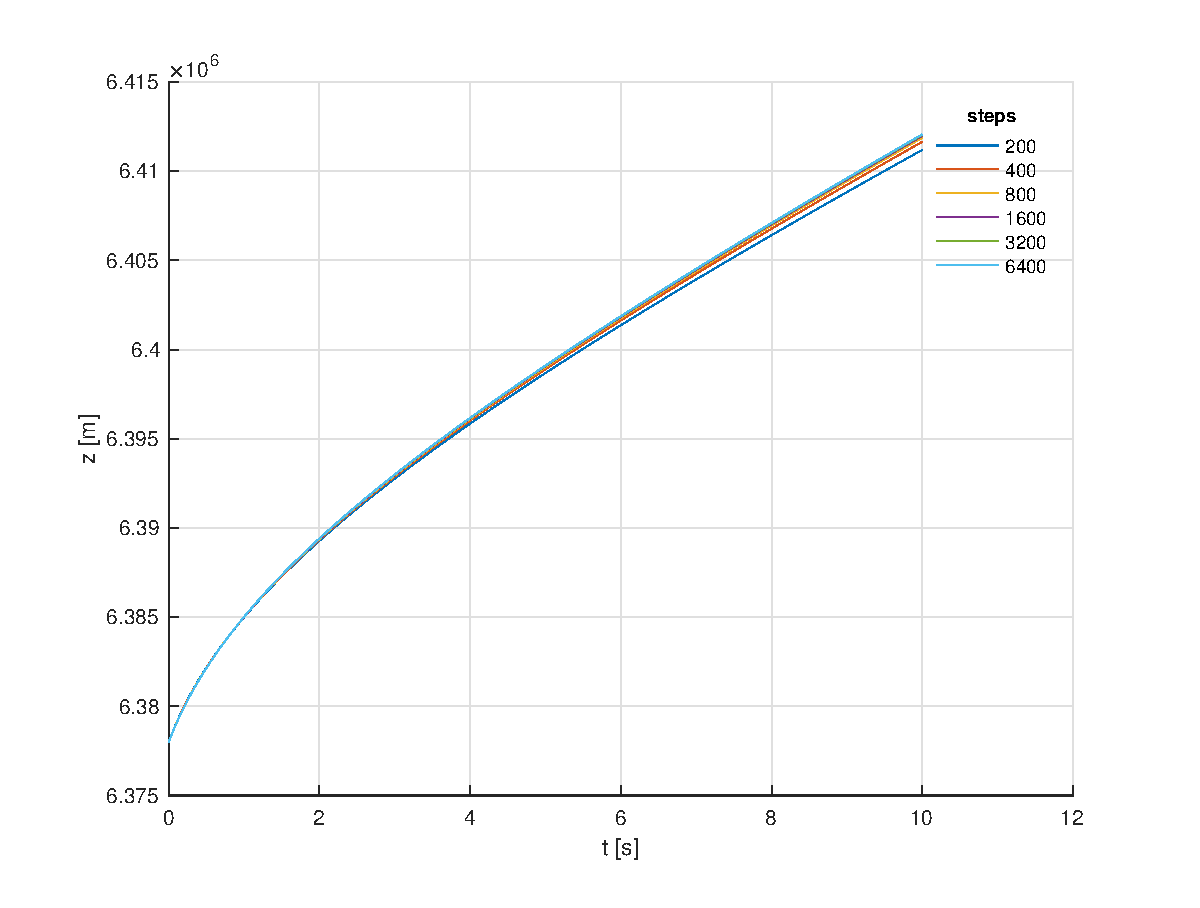
\includegraphics[width=0.53\textwidth]{graphs/zB.eps}
	\caption{Position en fonction du temps}
	\label{fig:B-zt}
\end{figure}

Concernant la tendance de l'accélération à tendre vers 0 provient du terme exponentiel de cette même force. Ce terme provient du calcul de la densité de l'air A VERIFIER, et il change de manière exponentielle lorsque la position change. Les paramètres gravitationnels se retrouvent aussi dans ces graphiques, mais ils agissent sur le projectile de la même manière qu'à la question A, donc nous n'en parlerons pas plus ici.
Toutes ces changements sur la vitesse grandement la position de l'objet. Ainsi, sur la figure \ref{fig:B-zt}, on observe que la position du projectile augmente drastiquement au début, mais ralenti rapidement son ascensions en deux secondes, pour finalement augmenter de manière plus ou moins constante sur la fin. Ainsi, au bout de 10 secondes, le projectile atteint une altitude d'environ \SI{40}{\kilo\meter} par rapport au sol terrestre.\\

\begin{figure}[h]
	\centering
	\begin{subfigure}[b]{0.45\textwidth}
		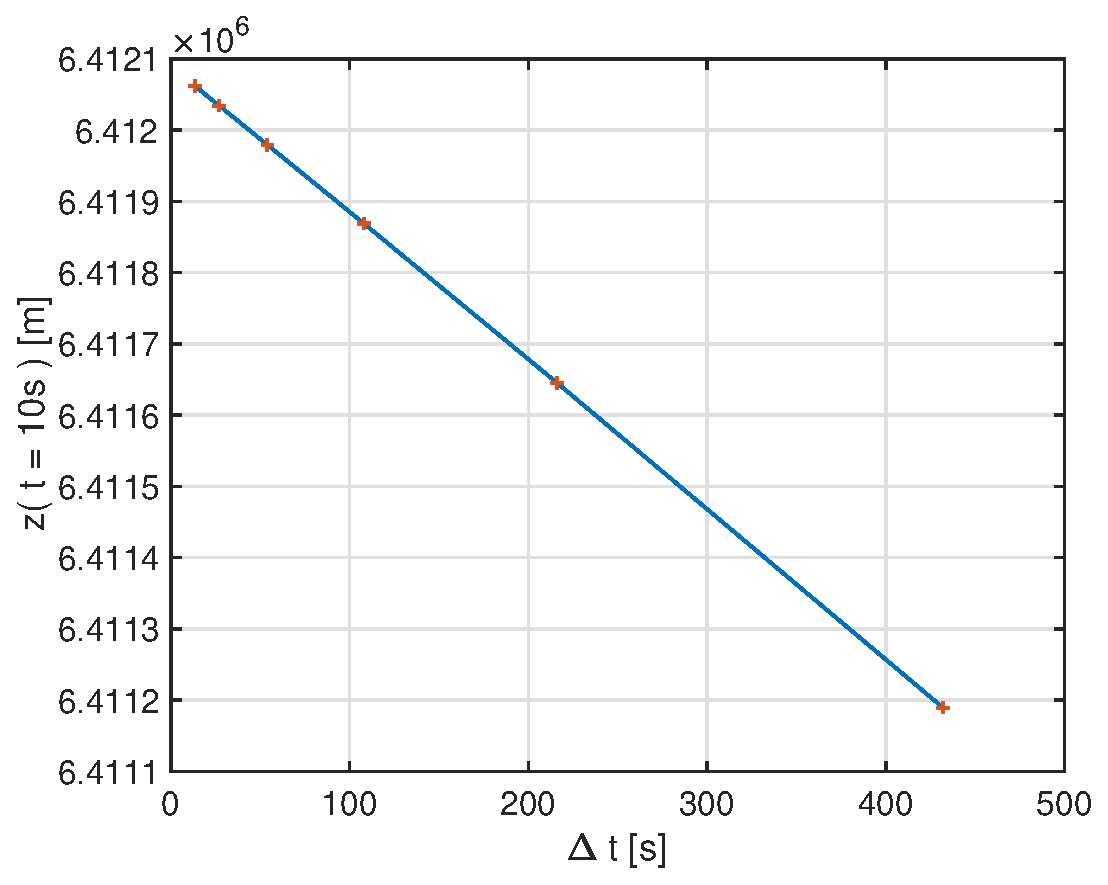
\includegraphics[width=\textwidth]{graphs/zConvB.eps}
		\caption{Graphique de convergence de la position}
		\label{fig:B-zConv}
	\end{subfigure}
	~
	\begin{subfigure}[b]{0.45\textwidth}
		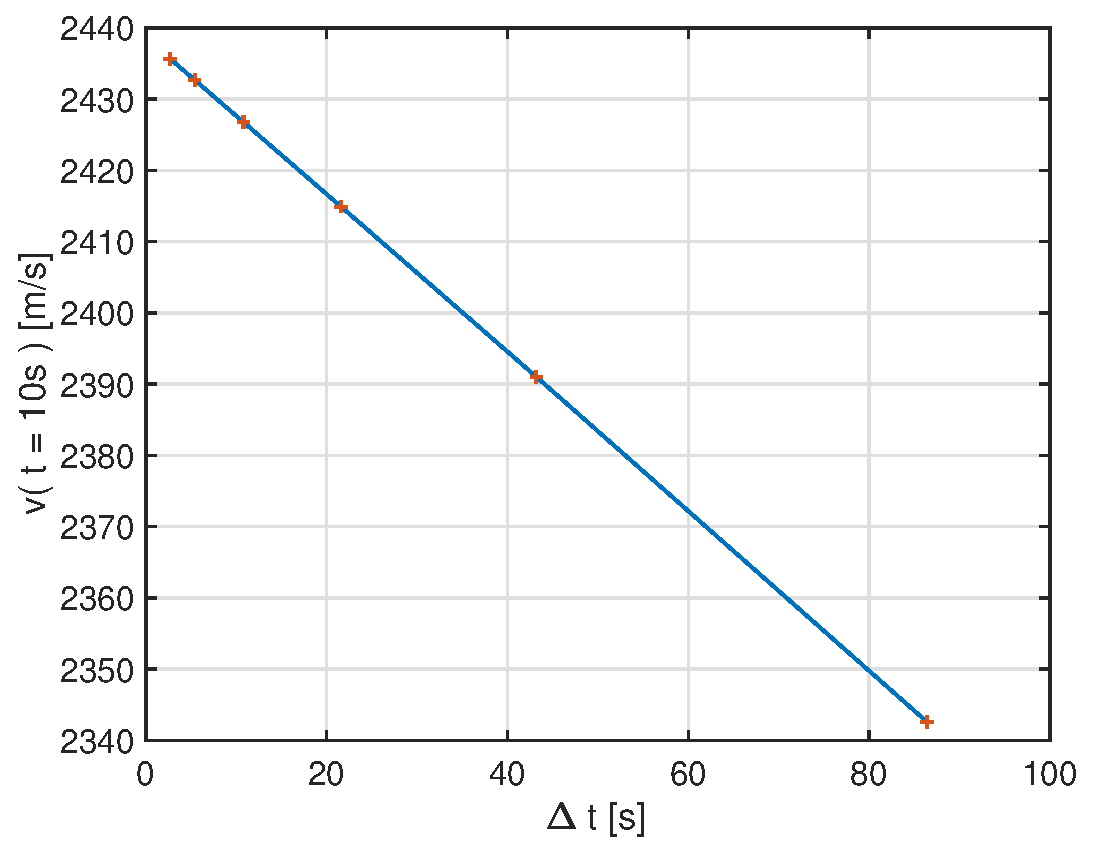
\includegraphics[width=\textwidth]{graphs/vConvB.eps}
		\caption{Graphique de convergence de la vitesse}
		\label{fig:B-vConv}
	\end{subfigure}
	\caption{Graphiques d'étude de convergence}
	\label{fig:B-conv}
\end{figure}

Dans les deux graphiques précédents (\ref{fig:B-vt} et \ref{fig:B-zt}), il semble que le nombre d'itérations de chaque simulation ne change pas drastiquement le déroulement de la simulation, du moins sur les 10 premières secondes. Il n'y a qu'un léger écart notoire entre les différents cas. Sur la figure \ref{fig:B-conv}, nous pouvons remarquer que les valeurs convergent vers une certaine vitesse ou position finale, en fonction du nombre d'itérations. À partir de ces deux graphiques, nous pouvons remarquer que le nombre d'itérations importe dans nos simulations. Plus le nombre d'itérations est important, plus la valeur finale va tendre vers la solution. Il n'y a donc pas de problème majeur dans l'utilisation de la méthode d'Euler pour résoudre numériquement l'équation différentielle \ref{eq:sol}.

\subsection{Question C - Bonus}

\section{Conclusion}

\end{document}